% --------------------------------------------------------------------------- %
\documentclass[a1paper,portrait]{baposter}

\usepackage{relsize}		% For \smaller
\usepackage{url}			% For \url
\usepackage{epstopdf}	% Included EPS files automatically converted to PDF to include with pdflatex

%%% Global Settings %%%%%%%%%%%%%%%%%%%%%%%%%%%%%%%%%%%%%%%%%%%%%%%%%%%%%%%%%%%

\graphicspath{{pix/}}	% Root directory of the pictures
\tracingstats=2			% Enabled LaTeX logging with conditionals

%%% Color Definitions %%%%%%%%%%%%%%%%%%%%%%%%%%%%%%%%%%%%%%%%%%%%%%%%%%%%%%%%%

\definecolor{bordercol}{RGB}{40,40,40}
\definecolor{headercol1}{RGB}{180,210,230}
\definecolor{headercol2}{RGB}{120,120,120}
\definecolor{headerfontcol}{RGB}{0,0,0}
\definecolor{boxcolor}{RGB}{220,240,220}

%%%%%%%%%%%%%%%%%%%%%%%%%%%%%%%%%%%%%%%%%%%%%%%%%%%%%%%%%%%%%%%%%%%%%%%%%%%%%%%%
%%% Utility functions %%%%%%%%%%%%%%%%%%%%%%%%%%%%%%%%%%%%%%%%%%%%%%%%%%%%%%%%%%

%%% Save space in lists. Use this after the opening of the list %%%%%%%%%%%%%%%%
\newcommand{\compresslist}{
	\setlength{\itemsep}{1pt}
	\setlength{\parskip}{0pt}
	\setlength{\parsep}{0pt}
}

%%%%%%%%%%%%%%%%%%%%%%%%%%%%%%%%%%%%%%%%%%%%%%%%%%%%%%%%%%%%%%%%%%%%%%%%%%%%%%%
%%% Document Start %%%%%%%%%%%%%%%%%%%%%%%%%%%%%%%%%%%%%%%%%%%%%%%%%%%%%%%%%%%%
%%%%%%%%%%%%%%%%%%%%%%%%%%%%%%%%%%%%%%%%%%%%%%%%%%%%%%%%%%%%%%%%%%%%%%%%%%%%%%%

\begin{document}
\typeout{Poster rendering started}

%%% Setting Background Image %%%%%%%%%%%%%%%%%%%%%%%%%%%%%%%%%%%%%%%%%%%%%%%%%%
\background{
	\begin{tikzpicture}[remember picture,overlay]%
	\draw (current page.north west)+(-2em,2em) node[anchor=north west]
	{\includegraphics[height=1.1\textheight]{background}};
	\end{tikzpicture}
}

%%% General Poster Settings %%%%%%%%%%%%%%%%%%%%%%%%%%%%%%%%%%%%%%%%%%%%%%%%%%%
%%%%%% Eye Catcher, Title, Authors and University Images %%%%%%%%%%%%%%%%%%%%%%
\begin{poster}{
	grid=false,
	% Option is left on true though the eyecatcher is not used. The reason is
	% that we have a bit nicer looking title and author formatting in the headercol
	% this way
	%eyecatcher=false,
	borderColor=bordercol,
	headerColorOne=headercol1,
	headerColorTwo=headercol2,
	headerFontColor=headerfontcol,
	% Only simple background color used, no shading, so boxColorTwo isn't necessary
	boxColorOne=boxcolor,
	headershape=roundedright,
	headerfont=\Large\sf\bf,
	textborder=rectangle,
	background=user,
	headerborder=open,
  boxshade=plain
}
%%% Eye Cacther %%%%%%%%%%%%%%%%%%%%%%%%%%%%%%%%%%%%%%%%%%%%%%%%%%%%%%%%%%%%%%%
{
	Eye Catcher, empty if option eyecatcher=false - unused
}
%%% Title %%%%%%%%%%%%%%%%%%%%%%%%%%%%%%%%%%%%%%%%%%%%%%%%%%%%%%%%%%%%%%%%%%%%%
{\sf\bf
    Coerction Game Master
}
%%% Authors %%%%%%%%%%%%%%%%%%%%%%%%%%%%%%%%%%%%%%%%%%%%%%%%%%%%%%%%%%%%%%%%%%%
{
	\vspace{0.5em} Group33: Liang-Wei Chen, John McCann, Yao-Yuan Yang, Hsiao-Ling Wang\\
}
%%% Logo %%%%%%%%%%%%%%%%%%%%%%%%%%%%%%%%%%%%%%%%%%%%%%%%%%%%%%%%%%%%%%%%%%%%%%
%{
%% The logos are compressed a bit into a simple box to make them smaller on the result
%% (Wasn't able to find any bigger of them.)
%\setlength\fboxsep{0pt}
%\setlength\fboxrule{0.5pt}
%	\fbox{
%		\begin{minipage}{14em}
%			\includegraphics[width=10em,height=4em]{colbud_logo}
%			\includegraphics[width=4em,height=4em]{elte_logo} \\
%			\includegraphics[width=10em,height=4em]{dynanets_logo}
%			\includegraphics[width=4em,height=4em]{aitia_logo}
%		\end{minipage}
%	}
%}

\headerbox{Problem}{name=problem,column=0,row=0}{
This project involves design, evaluate and analysis of intellegent agents for
the Queue ICPC Challenge game, Coercion.
}

\headerbox{Game Introduction}{name=game-intro,column=0,below=problem}{
The game Coercion is played in an environment like the following figure.
Red and blue players compete to coerce regions to their own color.
The one with the most region wins.

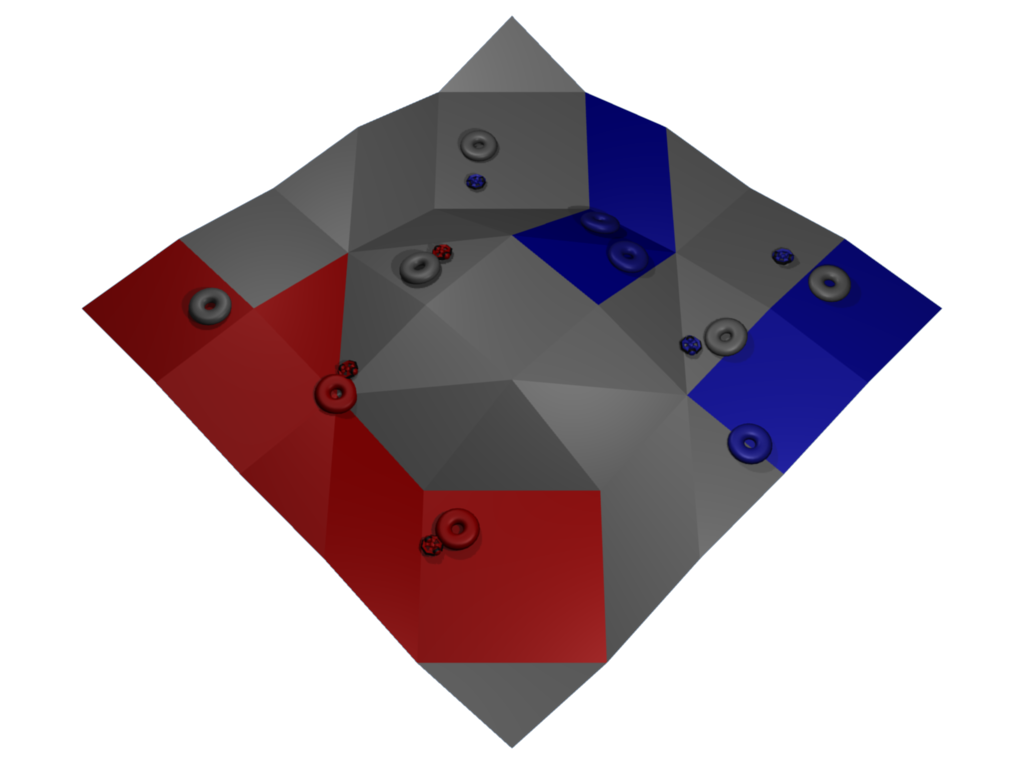
\includegraphics[width=0.99\linewidth]{game}
}

\headerbox{Rules}{name=rules,column=0,below=game-intro}{
\textbf{Pushers} Each player controls three pieces called pushers. \\
\textbf{Markers} The 22 markers may be moved by pushers. \\
\textbf{Color Coercion}
Enough markers touching a region can coerce the region to marker's color.
If a marker stays inside region of a different color, the marker can be
coerced to that region's color. \\

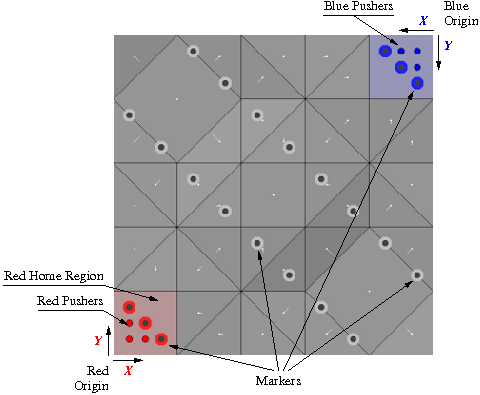
\includegraphics[width=0.99\linewidth]{initial}
}

\iffalse
\headerbox{Discussion}{name=discussion,column=0,below=rules, above=bottom}{
\smaller						% Make the whole text smaller
\vspace{-0.4em}			% Save some space at the beginning
} 
\fi

\headerbox{Agents}{name=agents,span=2,column=1,row=0}{

\textbf{Gather}Push as many markers to home region as possible.
\vspace{-0.6em}			% Save some space at the beginning
\begin{enumerate} \itemsep1pt \parskip0pt \parsep0pt
  \item Randomly choose a marker
  \item If not my marker: push it to home region
  \item Else: push it to a random region
\end{enumerate}
\vspace{-0.4em}

\textbf{Migrate} Spread out our markers from home region.
\vspace{-0.6em}			% Save some space at the beginning
\begin{itemize} \itemsep0pt \parskip0pt \parsep0pt
  \item Find out regions with both our vertices and not our vertices. Then push our
  markers to these regions.
\end{itemize}
\vspace{-0.4em}

\textbf{Robber} Rob enemy's markers as top priority
\vspace{-0.6em}			% Save some space at the beginning
\begin{enumerate} \itemsep0pt \parskip0pt \parsep0pt
  \item Randomly choose push an opponent's marker to home region.
  \item If enemy has no marker, push one of my marker to a random  region.
\end{enumerate}
\vspace{-0.4em}

\textbf{Greedy} Greedy agent based on the utility function
\vspace{-0.6em}			% Save some space at the beginning
\begin{itemize} \itemsep0pt \parskip0pt \parsep0pt
  \item Search space : All possbile (target region, marker) combinations
  \item Utility function : $10*(1-t)*num_{RedMarkers}-(1-t)*num_{BlueMarker}+20*t*num_{RedRegion}-20*t*num_{BlueRegion}$, where $t$ is the round number.
\end{itemize}
\vspace{-0.4em}

\textbf{Gather-migrate(GM)} Migrate existing markers while also gathering new markers into home regions
\vspace{-0.6em}			% Save some space at the beginning
\begin{enumerate} \itemsep0pt \parskip0pt \parsep0pt
  \item if gathering:
push nearest neutral or opposing marker into the closest home region.
  \item else:
push marker nearest home to an outside region.
\end{enumerate}
\vspace{-0.6em}

\textbf{enhancedRobber(eR)}: rob enemy's markers at top priority
\vspace{-0.6em}			% Save some space at the beginning
\begin{enumerate} \itemsep0pt \parskip0pt \parsep0pt
  \item Push the nearest enemy marker to my home region
  \item if enemy has no marker:  Push the nearest red marker to gray region and
      nearest gray marker to home.
\end{enumerate}
\vspace{-0.5em}
}

\headerbox{Evaluation}
{name=evaluation,span=2,column=1,below=agents}{
\vspace{-0.2em}
To evaluate our performance, we performs experiments by competing each of
our agents with each other. The following table is the result of the average of the score of
5 experiments:
\begin{center}
    \smaller[3]
    \begin{tabular}{ | c | c | c | c | c | c | c |}
    \hline
           & Gather       & Migrate   & Greedy   & Robber    & GM        & eR \\ \hline
    Gather & -            & 2440:1040 & 720:1960 & 480:2080  & 920:3960  & 840:2800  \\ \hline
    Migrate& 1040:2440    & -         & 400:1760 & 640:1120  & 1840:2200 & 760:2500  \\ \hline
    Greedy & 1960:720     & 1760:400  & -        & 400:400   & 1200:3200 & 600:800   \\ \hline
    Robber & 2080:480     & 1120:640  & 400:400  & -         & 1000:1200 & 380:720   \\ \hline
    GM     & 3960:920     & 2200:1840 & 3200:1200& 1200:1000 & -         & 800:4600\\ \hline
    eR     & 2800:840     & 2560:760  & 800:600  & 720:380   & 4600:800  & - \\ \hline
    \end{tabular}
\end{center}
}

\headerbox{Conclusion}
{name=conclusion,span=2,column=1,below=evaluation,above=bottom}{
\vspace{1em}
\begin{itemize} \itemsep0pt \parskip0pt \parsep0pt
  \item Approximate continuous spatial data with discrete inforamtion.
  \item Designed several huristic agents and agents based on utility function.
 Then we compare their performances by competeing.
  \item The greedy agent is the most stable and better performed agent compared with others.
\end{itemize}
}

\end{poster}
\end{document}
